\documentclass[output=paper,modfonts,nonflat]{langsci/langscibook} 

\title{Comparing bilingual word embeddings to translation dictionaries for extracting multilingual collocation equivalents}
\author{ Marcos Garcia\affiliation{Universidade da Coruña}}

\abstract{  This chapter introduces a strategy for the automatic extraction of multilingual  collocation equivalents which takes advantage of parallel corpora to train   bilingual word embeddings. First, monolingual collocation candidates are retrieved  using syntactic dependencies and standard association measures. Then, the distributional   models are applied to search for equivalents of the elements of each collocation in the target languages.  The proposed method extracts not only collocation equivalents with direct translations   between languages, but also other cases where the collocations in the two languages  are not literal translations of each other. Several experiments -- evaluating collocations   with five syntactic patterns -- in English, Spanish, and Portuguese show that this  approach can effectively extract large sets of bilingual equivalents with an average   precision of about $85\%$. Moreover, preliminary results on comparable corpora suggest  that the distributional models can be applied for identifying new bilingual collocations   in different domains. This strategy is compared to both hand-crafted bilingual dictionaries  and to probabilistic translation dictionaries learned from the same resources as the   bilingual word embeddings, showing that it achieves much larger recall values  while keeping high precision results.}

\begin{document}
\shorttitlerunninghead{Word embeddings and translation dictionaries in collocation extraction}%Needed to make the authors' headline shorter. Always place just after 
\maketitle
\label{GARCIA-CHAPTER}

\section{Introduction}
MWEs have been repeatedly classified as an important problem for developing
Natural Language Processing (NLP) tools, as well as to automatically analyze linguistic
utterances \citep{Sag2002a}. Among the different types of MWEs, processing
collocations in an automatic way may pose various problems due to their intrinsic properties
such as compositionality or unpredictability \citep{melcuk98}.

From a theoretical perspective, there are at least two main views on collocations.
On the one hand, there is a tendency to consider any frequent pair of words to be
a \isi{collocation} \citep{smadja1993,evert2003,kilgarriff2006}.
On the other hand, the phraseological tradition needs both a lexical restriction and a syntactic
relation to consider two lexical units as a \isi{collocation}.\footnote{An overview of different views on collocations
  -- both from theoretical and practical perspectives -- can be found in \citet{seretan2011syntax}.}
From this phraseological point of view, a \isi{collocation} is a restricted binary co-occurrence of lexical units
between which a syntactic relation holds, and that one of the lexical units (the \textsc{base})
is chosen according to its meaning as an isolated lexical unit, while the other (the \textsc{collocate})
is selected depending on the base and the intended meaning of the co-occurrence as a whole,
rather than on its meaning as an isolated lexical unit \citep{melcuk98}. Thus, a noun in \ili{English}
such as \ile{picture} (as a direct object) requires the verb \ile{to take} (and not \ile{to do}, or \ile{to make})
in the phrase \ile{take a picture}, while \ile{statement} selects \ile{to make} (\ile{make a statement}).

In a bilingual (or multilingual) scenario, equivalent collocations are needed
to produce more natural utterances in the target language(s). In this regard,
the referred noun \exidio{fotografia}{picture} would select the verb \exidio{tirar}{to remove} in \ili{Portuguese} (\ile{tirar uma fotografia}). Similarly the \ili{Spanish} \exidio{vino}{wine} would require the adjective \ile{tinto} (\ile{vino tinto}), which is not
the main translation of \ile{red} (\ile{red wine}).

The unpredictability of these structures poses problems for tasks such as
\isi{machine translation}, whose performance can benefit from lists of multilingual
collocations or transfer rules for these units \citep{orliac2003}.
In areas like second \isi{language learning}, it has been shown that even advanced learners
need to know which word combinations are allowed in a specific linguistic
variety \citep{altenberg2001,ramos2010}. Thus, obtaining resources of multilingual
equivalent collocations could be useful for a variety of applications such as those
mentioned above. However, this kind of resource is scarce, and constructing
them manually requires a large effort from expert lexicographers.

Since the 1990s, a number of approaches were implemented aimed at extracting
bilingual collocations, both from \isi{parallel corpora} \citep{kupiec1993,smadja1996,wu2003},
and from comparable or even from non-related monolingual resources \citep{lu2004,Rivera2013},
often combining statistical approaches with the use of bilingual dictionaries to
find equivalents of each base.

\newpage 
This chapter explores the use of \isi{distributional semantics} (by means of bilingual
\isi{word embeddings}) for identifying bilingual equivalents of monolingual collocations:
On the one hand, monolingual \isi{collocation} candidates are extracted using a harmonized
syntactic annotation provided by Universal Dependencies (UD),\footnote{\scriptsize{\url{http://universaldependencies.org/}}}
as well as standard measures for lexical association. On the other hand, bilingual
\isi{word embeddings} are trained using lemmatized versions of noisy \isi{parallel corpora}.
Finally, these bilingual models are employed to search for semantic equivalents of both
the base\is{collocation!base} and the collocate\is{collocation!collocate} of each \isi{collocation}.

Several experiments using the OpenSubtitles2016 \isi{parallel corpora} \citep{opus} in \ili{English},
\ili{Portuguese}, and \ili{Spanish}  show that the proposed method successfully
identifies bilingual \isi{collocation} equivalents with different patterns: \emph{adjective-noun},
\emph{noun-noun}, \emph{verb-object}, \emph{verb-subject}, and \emph{verb-adverb}.
Furthermore, preliminary results in comparable corpora suggest that the same strategy
can be applied in this kind of resources to extract new pairs of bilingual
collocations. In this regard, this chapter is an extended version of a previous work
on bilingual \isi{collocation} extraction \citep{mwe17}, including new \isi{collocation}
patterns and a larger evaluation which compares the proposed approach to probabilistic
translation dictionaries \citep{hiemstra1998,natools}.

Apart from this introduction, \sectref{garcia:sec:rw} includes a review of previous work on \isi{collocation}
extraction, especially on papers dealing with bilingual resources. Then, \sectref{garcia:sec:method}
and \sectref{garcia:sec:experiments} present and evaluate the method, respectively. Finally, some conclusions
and further work are discussed in \sectref{garcia:sec:conclusions}.


%
\section{Previous studies on collocation extraction}
\label{garcia:sec:rw}

The extraction of monolingual \isi{collocation} candidates (as well as other MWEs)
from corpora is a well-known topic in corpus and computational linguistics and was the focus of a significant body of work in different languages.

In this respect, most strategies use statistical association measures on windows of
n-grams with different sizes \citep{church1990, smadja1993}. Other methods, such as the
one presented by \citet{lin1999}, started to apply dependency parsing\is{parsing!dependency} to better identify
combinations of words which occur in actual syntactic relations.

More recently, the availability of better parsers allowed researchers to combine automatically
obtained syntactic information with statistical methods to extract collocations more accurately \citep{evert2008,seretan2011syntax}.

A different perspective on \isi{collocation} extraction focuses not only on their retrieval, but on
semantically classifying the obtained collocations, in order to make them more useful for NLP
applications \citep{wanner2006,wanner2016}.

Concerning the extraction of bilingual collocations, most works rely on \isi{parallel corpora} to find the
equivalent of a \isi{collocation} in a target language. In this regard, \citet{smadja1992} and \citet{smadja1996}
first identify monolingual collocations in \ili{English} (the source language), and then use \textsc{Mutual
  Information} (\textsc{mi}) and the \textsc{Dice coefficient} to find the \ili{French} equivalents of the source
collocations. 

\citet{kupiec1993} also uses \isi{parallel corpora} to find noun phrase equivalents between \ili{English}
and \ili{French}. Their method consists of applying an expectation maximization (EM) algorithm to previously
extracted monolingual collocations.
Similarly, \citet{haruno1996} obtain Japanese-\ili{English} chunk equivalents by computing
their \textsc{mi} scores and taking into account their frequency and position in the aligned corpora.

Another work which uses \isi{parallel corpora} is presented by \citet{wu2003}. The authors
extract Chinese and \ili{English} n-grams from aligned sentences by computing their \textsc{log-likelihood} ratio.
Then, the competitive linking algorithm is used to decide whether each bilingual pair actually
corresponds to a translation equivalent.

\citet{seretan2007} took advantage of syntactic parsing to extract bilingual collocations from \isi{parallel corpora}.
The strategy consists of first extracting monolingual collocations using log-likelihood,
and then searching for equivalents of each base using bilingual dictionaries.
The method also uses the position of the \isi{collocation} in the corpus, and relies on the syntactic analysis
by assuming that equivalent collocations will occur with the same syntactic relations within the collocations in both languages.

\citet{Rivera2013} present a framework for bilingual \isi{collocation} retrieval
that can be applied (using different modules) to both parallel and comparable corpora.
As in other works, monolingual collocations based on n-grams are extracted in a first
step, and then bilingual dictionaries (or WordNet, in the comparable corpora scenario) are used
to find the equivalents of the base in the aligned sentence or in a small window of
adjacent sentences of the source \isi{collocation}.

\largerpage
A different approach, which uses non-related monolingual corpora for finding bilingual
collocations, was presented in \citet{lu2004}. Here, the authors apply dependency parsing
and the log-likelihood ratio for obtaining \ili{English} and Chinese collocations. Then,
they search for translations using word translation equivalents with the same dependency
relation\is{dependency!relation} in the target language (using the EM algorithm and a bilingual dictionary).

Although not focused on collocations, \citet{fung1998} applied methods based on distributional
semantics to build bilingual lexica from comparable corpora.
This approach takes into account that in this type of resources the position and the frequency
of the source and target words are not comparable, and also that the translations of the source
words might not exist in the target document.

Similarly, the strategy presented in this chapter leverages noisy \isi{parallel corpora} for building
bilingual \isi{word embeddings}. However, with a view to applying it to other resources such as comparable corpora, it identifies equivalents without using information about the position of the collocations
or their comparative frequency in the corpora. Furthermore, it does not take advantage
of external resources such as bilingual dictionaries, making it easy to extend to other languages.
\citet{pacorbook} had introduced a naive version of this approach, including experiments in \ili{Portuguese} and \ili{Spanish} with just one \isi{collocation} pattern.


%
\section{A new method for bilingual collocation extraction}
\label{garcia:sec:method}
This section presents the proposed method for automatically extracting bilingual collocations from corpora.
First, the approach for identifying candidates of monolingual collocations using syntactic dependencies
is briefly described. Then, the process of creating the bilingual \isi{word embeddings} is shown,
followed by the strategy for discovering the \isi{collocation} equivalents between languages.

%
\subsection{Monolingual dependency-based collocation extraction}
\label{garcia:sec:monolingual}
Early works on n-gram based \isi{collocation} extraction already pointed out the
need for syntactic analysis to better identify collocations in corpora
\citep{smadja1993,lin1999}. Syntactic analysis can, on the one hand, avoid the
extraction of syntactically unrelated words which occur in small context
windows. On the other hand, it can effectively establish a relation
between lexical items occurring in long-distance dependencies \citep{evert2008}.

Besides, the method presented
in this chapter assumes that most bilingual equivalents of collocations bear the same syntactic
relation in both the source and the target languages, although it is not always the case \citep{lu2004}.

In order to better capture the syntactic relations between the base and
the collocate of each \isi{collocation}, the strategy uses state-of-the-art dependency
parsing\is{parsing!dependency}. Apart from that, and aimed at obtaining harmonized syntactic information
between languages, the method relies on Universal Dependencies\is{Universal Dependencies} annotation,
which makes it possible to use the same strategy for extracting and analyzing the collocations in multiple
languages.%\footnote{\scriptsize{\url{http://universaldependencies.org/u/dep/all.html}}}

\subsubsection{Preprocessing:} Before extracting the collocation candidates from each
corpus, a pipeline of NLP tools is applied in order to annotate the text with the
desired information. Thus, the output of this process consists of a parsed corpus
in CoNLL-U format,\footnote{\scriptsize{\url{http://universaldependencies.org/format.html}}} where each word is assigned to its surface form, its lemma, its
POS-tag and morphosyntactic features, its syntactic head as well as the UD
relation of the word in context.

From this analyzed corpus, the word pairs belonging to the desired relations
(\isi{collocation} candidates) are extracted. We keep their surface forms, POS-tags,
and other syntactic dependents which may be useful for the identification
of potential collocations. Besides, a list of triples is retained in order to apply association measures,
containing (i) the syntactic relation, (ii) the head, and (iii) the dependent (using their lemmas
together with the POS-tags). Thus, from a sentence such as \emph{John took a great responsibility},
the following triples (among others) are obtained:

\begin{quotation}
  \noindent\textsc{nsubj}(take\textsubscript{\textsc{Verb}},John\textsubscript{\textsc{PropN}})\\
  \textsc{amod}(responsibility\textsubscript{\textsc{Noun}},great\textsubscript{\textsc{Adj}})\\
  \textsc{dobj}(take\textsubscript{\textsc{Verb}},responsibility\textsubscript{\textsc{Noun}})
\end{quotation}

This information, along with the corpus size and the frequency of the different elements
of the potential collocations, is stored in order to rank the candidates.

\subsubsection{Collocation patterns:} In this chapter, candidates of five different syntactic
patterns of collocations are extracted in three languages, \ili{Spanish} (ES), \ili{Portuguese} (PT), and \ili{English} (EN):\footnote{In this chapter we address the European variety of Portuguese.
  However, even if we use a European Portuguese corpus (see \sectref{garcia:sec:experiments}),
  it contains some texts in the Brazilian dialect.}

\begin{itemize}
\item Adjective---Noun (\textsc{amod}): these candidates are pairs of adjectives
(as collocates) and nouns (as bases) where the former syntactically depends
of the latter in a \textsc{amod} relation.
Example: \textbf{killer}\textsubscript{base};\textbf{serial}\textsubscript{collocate}.

\item Noun---Noun (\textsc{nmod}): this pattern consists of two common
nouns related by the \textsc{nmod} relation, where the head is the base
and the dependent is the collocate (optionally with a \textsc{case} marking
dependent preposition: \emph{of} in \ili{English}, \emph{de} in \ili{Portuguese} and \ili{Spanish}).
Example: \textbf{rage}\textsubscript{base};\textbf{fit}\textsubscript{collocate}.\footnote{Some
  collocations belonging to this pattern are analyzed in UD -- mainly in English --
  using the \textsc{compound} relation. These are not extracted in the experiments performed in this chapter.}

\item Verb---Object (\textsc{vobj}): \emph{verb-object} collocations consist
of a verb (the collocate) and a common noun (the base)
occurring in a \textsc{dobj} relation.
Example: \textbf{care}\textsubscript{base};\textbf{take}\textsubscript{collocate}.

\item Subj---Verb (\textsc{vsubj}): the \textsc{vsubj} collocation pattern contains a
  common noun (the base, acting as a subject) and the verb it depends on
  (the collocate).
  Example: \textbf{ship}\textsubscript{base};\textbf{sink}\textsubscript{collocate}.
  
\item Verb---Adverb (\textsc{advmod}): in this case, a collocate adverb modifies
  a verb (the base) in an \textsc{advmod} relation.
  Example: \textbf{want}\textsubscript{base};\textbf{really}\textsubscript{collocate}.
\end{itemize}

\subsubsection{Identification of candidates:} For each of the five patterns of
collocations, a list of potential candidates for the three languages is extracted.
After that, the candidates are ranked using standard association measures that have
been widely used in collocation extraction \citep{evert2008}.

In the current experiments, two statistical measures were selected, whose results
complement each other: \textsc{t-score}, which prefers frequent dependency pairs,
and has been proved useful for collocation extraction \citep{krenn2001}, and
\textsc{Mutual Information}, which is useful for a large corpus, even if it
tends to assign high scores to candidates with very low-frequency \citep{pecina2010lexical}.

The output of both association measures is merged in a final list for each
language and collocation pattern, defining thresholds of \emph{\textsc{t-score$\geq$2}} and
\emph{\textsc{mi}$\geq$3}~\citep{stubbs1995}, and extracting only collocations with a frequency
of \emph{f$\geq$10}. This large value was defined to reduce the extraction of incorrect
entries from a noisy corpus and from potential errors of the automatic analysis.

It must be noted that, since these lists of monolingual collocations have been built
based on statistical measures of collocability, their members need not be
\emph{bona fide} collocations in the phraseological meaning. Thus, the lists can include
idioms, e.g., \ile{kick the bucket}, quasi-idioms, e.g., \ile{big deal}, \citep{melcuk98}, or free combinations, e.g., \ile{buy a drink}.

%
\subsection{Bilingual word embeddings}
\label{garcia:sec:models}
Word embeddings are low-dimensional vector representations of words which
capture their distributional context in corpora. Even though distributional
semantics methods have been largely used in previous years, approaches based
on \isi{word embeddings} gained popularity with the publication of \emph{word2vec}~\citep{mikolov2013}.
Based on the \emph{Skip-gram} model of \emph{word2vec}, \citet{bivec} proposed
\emph{BiSkip}, a model of \isi{word embeddings} which learns bilingual representations
using aligned corpora, thus being able to predict words crosslinguistically.

The method presented in this chapter uses lemmas instead of surface forms to identify the
\isi{collocation} candidates, so the bilingual models of \isi{word embeddings} are also trained on
lemmatized corpora. Therefore, the raw parallel corpus is lemmatized keeping the original sentence alignment.

The bilingual models are built 
%(on the lemmatized version of the corpora) 
using \emph{MultiVec},
an implementation of \emph{word2vec} and \emph{BiSkip} \citep{MultiVec}. As the approach
is evaluated in three languages, three different bilingual models are needed:
\ili{Spanish}-\ili{English},  \ili{Portuguese}-\ili{English}, and \ili{Spanish}-{Portu\-guese}.

As it will be shown, the obtained models can predict the similarity between words
in bilingual scenarios by computing the cosine similarity between their vectors. As
the models learn the distribution of single words (lemmas), they deal with different
semantic phenomena such as polysemy or homonymy. Concerning collocations, this means
that, ideally, the bilingual models could predict not only the equivalents of a
base, but also to capture the (less close) semantic relation between the
bilingual collocates, if they occur frequently enough in the data.

%
\subsection{Bilingual collocation alignment}
\label{garcia:sec:align}
In order to identify the bilingual equivalent of a \isi{collocation} in a target language,
the method needs (i) lists of monolingual collocations (ideally obtained from similar
resources), and (ii) a bilingual \emph{source-target} model of \isi{word embeddings}.

With these resources, the following strategy is applied: For each \isi{collocation}
in the source language (e.g., \exidio{lío\textsubscript{base} tremendo\textsubscript{collocate}}{huge mess} in \ili{Spanish}) the system selects its base and obtains -- using the bilingual model --
the \emph{n} most similar lemmas in the target language (where \emph{n=5} in the experiments
performed in this chapter): \ile{trouble}, \ile{mess}, etc. Then, starting from the most similar lemma,
we search in the target list for collocations containing the equivalents of
the base (\ile{trouble}\textsubscript{base} \ile{little}\textsubscript{collocate},
\ile{trouble}\textsubscript{base} \ile{deep}\textsubscript{collocate}, \ile{mess}\textsubscript{base} \ile{huge}\textsubscript{collocate}, \ile{mess}\textsubscript{base} \ile{fine}\textsubscript{collocate}, etc.). If a \isi{collocation} with
a base equivalent is found, the cosine similarity between both collocates
(\ile{tremendo} versus \ile{little}, \ile{deep}, \ile{huge}, and \ile{fine}) is computed, and
they are selected as potential candidates if their similarity is higher than a given threshold
(empirically defined in this chapter as $0.65$), and if the target candidate is among the \emph{n}
most similar words of the source collocate (again, \emph{n=5}). Finally, if these conditions
are met, the source and target collocations are aligned, assigning the average distance between the
bases and the collocates as a confidence value, as in the following Spanish-English example:
\ile{lío\textsubscript{base} tremendo\textsubscript{collocate}} = \ile{mess\textsubscript{base} huge\textsubscript{collocate}} $\rightarrow$ 0.721.

%
\section{Evaluation}
\label{garcia:sec:experiments}
This section presents the experiments carried out in order to evaluate the proposed distributional
method (henceforth \textsc{DiS}) in the three analyzed languages, using the five \isi{collocation}
patterns defined in \sectref{garcia:sec:monolingual}. The approach presented in this chapter is
compared to a baseline system (\textsc{Bas}), which uses hand-crafted bilingual dictionaries,
and to probabilistic translation dictionaries (\textsc{Nat}).\footnote{The extractions
  of these three methods are available at {\url{http://www.grupolys.org/~marcos/pub/pmwe-dis.tar.bz2}}}

\paragraph*{Corpora:} Monolingual collocations were extracted from a subset of the
OpenSubtitles2016 corpus \citep{opus}, which contains \isi{parallel corpora} from TV and Movie
subtitles. This resource was selected because it is a large and multilingual parallel corpus
likely to contain different types of collocations, also from an informal register,
thus being useful for comparative studies.\footnote{Note, however, that
  OpenSubtitles2016 includes non-professional translations with some noisy elements such as typos
  or case inconsistencies, among others.}

From the \ili{English}, \ili{Spanish}, and \ili{Portuguese} corpora, those senteces which appear in the three
languages were selected, for a total of 13,017,016 sentences. These sentences were tokenized, lemmatized
and POS-tagged with a multilingual NLP pipeline~\citep{Citius}, obtaining three corpora of about $91$M (ES and PT), and about $98$M (EN) tokens. The resulting data
were enriched with syntactic annotation using statistical models trained with MaltParser \citep{MaltParser} on version 1.4 of the UD\is{Universal Dependencies} treebanks \citep{univdep}.

\begin{table} 
    %\setlength\tabcolsep{4pt}
        \caption{\label{tab:mono} Number of unique input dependencies for each syntactic pattern (\emph{deps}),
          and final monolingual collocation candidates (\emph{colls}).}
    \fittable{{
    \begin{tabular}{lrrrrrrrrrr}
      \lsptoprule
      \textbf{\multirow{2}{*}{Lg}} & \multicolumn{2}{c}{\textbf{\textsc{amod}}} & \multicolumn{2}{c}{\textbf{\textsc{nmod}}} & \multicolumn{2}{c}{\textbf{\textsc{vobj}}} & \multicolumn{2}{c}{\textbf{\textsc{vsubj}}} & \multicolumn{2}{c}{\textbf{\textsc{advmod}}} \\
      & \emph{deps} & \emph{colls} & \emph{deps} & \emph{colls} & \emph{deps} & \emph{colls} & \emph{deps} & \emph{colls} & \emph{deps} & \emph{colls}\\
      \midrule
      \emph{ES}   & 373K & 13,870   & 644K & 5,673   & 423K & 17,723 & 287K & 4,914 & 124K & 5,526 \\
      \emph{PT}   & 361K & 12,967   & 709K & 5,643   & 544K & 20,984 & 283K & 3,927 & 142K & 6,660 \\
      \emph{EN}   & 381K & 14,175   & 517K & 3,133   & 483K & 15,492 & 264K & 2,663 & 162K & 6,711 \\
      \lspbottomrule
    \end{tabular}
    }} 
\end{table}

\paragraph*{Collocations:} From each corpus, five patterns of \isi{collocation} candidates
were extracted: \textsc{amod}, \textsc{nmod}, \textsc{vobj}, \textsc{vsubj}, and \textsc{advmod}.
For each language and pattern, a single list of collocations was obtained by merging the \textsc{mi}
and \textsc{t-score} outputs as explained in \sectref{garcia:sec:monolingual}. \tabref{tab:mono}
shows the number of filtered collocations in each case (\emph{colls}).

Another version of each corpus was created only with the lemma of each token,
keeping the original sentence alignments. These corpora were used for training
three bilingual \isi{word embeddings} with MultiVec, with $100$ dimensions and
a window-size of eight words: ES-EN, ES-PT, and PT-EN.\footnote{These models are available at \scriptsize{\url{http://www.grupolys.org/~marcos/pub/mwe17_models.tar.bz2}}}

\paragraph*{Baseline (\textsc{Bas}):} The performance of the method described in \sectref{garcia:sec:align}
was compared to a baseline which follows the same strategy, but uses bilingual
dictionaries instead of the \isi{word embeddings} models. Thus, the \textsc{Bas} method obtains the
equivalents of both the base and the collocate of a source \isi{collocation},
and verifies whether there is a target \isi{collocation} with the translations. The bilingual
dictionaries provided by the \emph{apertium} project were used for
these experiments \citep{apertium}.\footnote{SVN revision 75,477, \scriptsize{\url{https://svn.code.sf.net/p/apertium/svn/}}}

The \ili{Spanish}-\ili{Portuguese} dictionary has $14,364$ entries, and the \ili{Spanish}-\ili{English} one
contains $34,994$. The \ili{Portuguese}-\ili{English} dictionary (not provided by \emph{apertium})
was automatically obtained by transitivity from the two other lexica, with
a size of $9,160$ pairs.

\paragraph*{Probabilistic translation dictionaries (\textsc{Nat}):} The distributional method
was also compared to probabilistic translation dictionaries. Probabilistic dictionaries are
bilingual resources which contain, for each word in a source language, possible translations
in the target language together with the probability of the translation being correct.
To obtain these dictionaries NATools was used, which is a set of tools to work with \isi{parallel corpora}
that can be utilized for different tasks such as sentence and word alignment, or to extract bilingual
translation dictionaries by means of statistical methods \citep{natools}. The probabilistic dictionaries
are obtained by applying the EM algorithm on sparse matrices of bilingual word co-occurrences, previously
built from \isi{parallel corpora}~\citep{hiemstra1998}.

For a better comparison to the \textsc{DiS} model, \textsc{Nat} dictionaries were
extracted from the same lemmatized resources used for training the bilingual \isi{word embeddings}.
Thus, this method only differs from \textsc{DiS} in the bilingual resources used to
search for equivalents of the bases and the collocates.\footnote{After preliminary
  evaluations, the translation probability thresholds of both lexical units were empirically defined as $0.1$.}

%
\subsection{Results}
With a view to knowing the performance of \textsc{Bas}, \textsc{Nat}, and \textsc{DiS}
in the different scenarios, $100$ bilingual \isi{collocation} pairs were randomly selected
from each language and pattern, creating a total of 45 lists (15 from each of the three methods).\footnote{Except for baseline extractions with less than $100$ elements, where all of them were selected.}

Three reviewers worked during the evaluation process. Each bilingual \isi{collocation}
pair was labeled as (i) correct, (ii) incorrect, or (iii) dubious, which includes pairs where the
translation might be correct in some contexts even if they were not considered faithful
translations.\footnote{Some of these dubious equivalents are actual translations in the
  original corpus, such as the Spanish-English \exidio{copa de champaña}{champagne cup}, which was translated as \ile{cup of wine},
  even if they are semantically different.}
Correct \isi{collocation} equivalents are those pairs where the monolingual extractions were
considered correct, both in terms of co-occurrence frequency and of \isi{collocation} pattern
\isi{classification}, and whose translations were judged by the reviewers as potential
translations in a real scenario.
Two reviewers labeled each collocation pair in the \textsc{Bas} and \textsc{DiS} outputs, achieving 92\% and 83\% \isi{inter-annotator agreement}, respectively, with an average $\kappa=0.39$, which
indicates the difficulty of this kind of annotation. Pairs with correct/incorrect disagreement
were discarded for the evaluation. Those with at least one dubious label were checked by a
third annotator, deciding in each case whether they were correct, incorrect, or dubious.
This third annotator evaluated the outputs of \textsc{Nat} using exactly the same guidelines.

\begin{table}
  \begin{center}
    %{\small{
    %\setlength\tabcolsep{4pt}
    \caption{\label{tab:extract} Number of bilingual extractions of the baseline,
      \textsc{Nat}, and \textsc{DiS} systems.}
    \begin{tabular}{llrrr}
      \lsptoprule
      \textbf{Pattern} & \textbf{model} & \textbf{ES-PT} & \textbf{ES-EN} & \textbf{PT-EN}\\
      \midrule
	\multirow{3}{*}{\textsc{amod}} & \textsc{Bas} & 657 & 248 & 213\\ 
	& \textsc{Nat} & 1,329 & 1,113 & 1,005\\ 
	& \textsc{DiS} & 9,464 & 7,778 & 7,083\\ \midrule
	\multirow{3}{*}{\textsc{nmod}} & \textsc{Bas} & 320 & 32 & 43\\ 
	& \textsc{Nat} & 704 & 138 & 136\\ 
	& \textsc{DiS} & 3,867 & 890 & 917\\ \midrule
	\multirow{3}{*}{\textsc{vobj}} & \textsc{Bas} & 529 & 183 & 241\\ 
	& \textsc{Nat} & 1,443 & 1,461 & 1,544\\ 
	& \textsc{DiS} & 12,887 & 8,865 & 9,206\\ \midrule
	\multirow{3}{*}{\textsc{vsubj}} & \textsc{Bas} & 188 & 27 & 55\\ 
	& \textsc{Nat} & 382 & 346 & 323\\ 
	& \textsc{DiS} & 2,522 & 1,344 & 1,298\\ \midrule
	\multirow{3}{*}{\textsc{advmod}} & \textsc{Bas} & 58 & 19 & 22\\ 
	& \textsc{Nat} & 113 & 104 & 106\\ 
	& \textsc{DiS} & 3,721 & 2,301 & 2,412\\
      \lspbottomrule
    \end{tabular}
    %}}
  \end{center}
\end{table}


\begin{table}
  \begin{center}
    \caption{\label{tab:bas} Precision, recall and f-score of the baseline (\textsc{Bas}) system (\emph{average} is macro-average).}
    \begin{tabular}{llrrrr}
      \lsptoprule
      \multicolumn{2}{l}{\textbf{Pattern}} & \textbf{ES-PT} & \textbf{ES-EN} & \textbf{PT-EN} & \textbf{average}\\
      \midrule
	\multirow{3}{*}{\textsc{amod}} & P & 99.0 & 95.8 & 97.9 & 97.6\\ 
	& R & 5.0 & 1.7 & 1.6 & 2.8\\ 
	& F1 & 9.6 & 3.4 & 3.2 & 5.4\\ \midrule
	\multirow{3}{*}{\textsc{nmod}} & P & 97.8 & 100\phantom{.0} & 91.7 & 96.5\\ 
	& R & 5.5 & 1.0 & 1.3 & 2.6\\ 
	& F1 & 10.5 & 2.0 & 2.5 & 5.1\\  \midrule
	\multirow{3}{*}{\textsc{vobj}} & P & 98.7 & 100\phantom{.0} & 92.1 & 96.9\\ 
	& R & 3.0 & 1.2 & 1.4 & 1.9\\ 
	& F1 & 5.7 & 2.3 & 2.8 & 3.6\\  \midrule
	\multirow{3}{*}{\textsc{vsubj}} & P & 93.8 & 96.3 & 92.7 & 94.3\\ 
	& R & 4.5 & 1.0 & 1.9 & 2.5\\ 
	& F1 & 8.6 & 1.9 & 3.8 & 4.8\\  \midrule
	\multirow{3}{*}{\textsc{advmod}} & P & 96.7 & 100\phantom{.0} & 95.7 & 97.4\\ 
	& R & 1.0 & 0.3 & 0.3 & 0.6\\ 
	& F1 & 2.0 & 0.7 & 0.6 & 1.1\\  \midrule
	\multirow{3}{*}{\emph{average}} & P & 97.2 & 98.4 & 94.0 & 96.5\\ 
	& R & 3.8 & 1.0 & 1.3 & 2.1\\ 
	& F1 & 7.3 & 2.1 & 2.6 & 4.0\\
      \lspbottomrule
    \end{tabular}
  \end{center}
\end{table}


\begin{table}
  \begin{center}
    \caption{\label{tab:nat} Precision, recall and f-score of the probabilistic (\textsc{Nat}) system (\emph{average} is macro-average).}
    \begin{tabular}{llrrrr}
      \lsptoprule
      \multicolumn{2}{l}{\textbf{Pattern}} & \textbf{ES-PT} & \textbf{ES-EN} & \textbf{PT-EN} & \textbf{average}\\
      \midrule
	\multirow{3}{*}{\textsc{amod}} & P & 92.5 & 92.5 & 83.3 & 89.5\\
	& R & 9.5 & 7.4 & 6.5 & 7.8\\
	& F1 & 17.2 & 13.8 & 12.0 & 14.3\\ \midrule
	\multirow{3}{*}{\textsc{nmod}} & P & 91.1 & 98.7 & 91.4 & 93.7\\
	& R & 11.4 & 4.4 & 4.0 & 6.6\\
	& F1 & 20.2 & 8.3 & 7.6 & 12.1\\ \midrule
	\multirow{3}{*}{\textsc{vobj}} & P & 95.2 & 80.0 & 92.7 & 89.3\\
	& R & 7.8 & 7.5 & 9.2 & 8.2\\
	& F1 & 14.3 & 13.8 & 16.8 & 15.0\\ \midrule
	\multirow{3}{*}{\textsc{vsubj}} & P & 82.4 & 78.6 & 79.2 & 80.0\\
	& R & 8.0 & 10.2 & 9.6 & 9.3\\
	& F1 & 14.6 & 18.1 & 17.1 & 16.6\\ \midrule
	\multirow{3}{*}{\textsc{advmod}} & P & 59.2 & 78.8 & 83.3 & 73.8\\
	& R & 1.2 & 1.5 & 1.3 & 1.3\\
	& F1 & 2.4 & 2.9 & 2.6 & 2.6\\ \midrule
	\multirow{3}{*}{\emph{average}} & P & 84.1 & 85.7 & 86.0 & 85.3\\
	& R & 7.6 & 6.2 & 6.1 & 6.6\\
	& F1 & 13.8 & 11.4 & 11.2 & 12.1\\
      \lspbottomrule
    \end{tabular}
  \end{center}
\end{table}


\begin{table}
  \begin{center}
    \caption{\label{tab:sys} Precision, recall and f-score of \textsc{DiS} system (\emph{average} is macro-average).}
    \begin{tabular}{llrrrr}
      \lsptoprule
      \multicolumn{2}{l}{\textbf{Pattern}} & \textbf{ES-PT} & \textbf{ES-EN} & \textbf{PT-EN} & \textbf{average}\\
      \midrule
	\multirow{3}{*}{\textsc{amod}} & P & 92.9 & 92.0 & 90.5 & 91.8\\ 
	& R & 67.8 & 51.6 & 49.5 & 56.3\\ 
	& F1 & 78.4 & 64.3 & 64.0 & 68.9\\ \midrule
	\multirow{3}{*}{\textsc{nmod}} & P & 93.8 & 88.0 & 90.0 & 90.6\\ 
	& R & 64.3 & 25.0 & 26.3 & 38.5\\ 
	& F1 & 76.3 & 38.9 & 40.1 & 51.9\\ \midrule
	\multirow{3}{*}{\textsc{vobj}} & P & 90.1 & 84.0 & 83.9 & 86.2\\ 
	& R & 66.0 & 48.1 & 49.9 & 54.7\\ 
	& F1 & 76.5 & 61.2 & 62.6 & 66.7\\ \midrule
	\multirow{3}{*}{\textsc{vsubj}} & P & 80.3 & 81.2 & 74.1 & 78.5\\ 
	& R & 51.6 & 41.0 & 36.1 & 42.9\\ 
	& F1 & 62.8 & 54.5 & 48.6 & 55.3\\ \midrule
	\multirow{3}{*}{\textsc{advmod}} & P & 77.6 & 83.3 & 67.4 & 76.1\\ 
	& R & 52.2 & 34.7 & 24.4 & 37.1\\ 
	& F1 & 62.4 & 49.0 & 35.8 & 49.1\\ \midrule
	\multirow{3}{*}{\emph{average}} & P & 86.9 & 85.7 & 81.2 & 84.6\\ 
	& R & 60.4 & 40.1 & 37.3 & 45.9\\ 
	& F1 & 71.3 & 53.6 & 50.2 & 58.4\\
      \lspbottomrule
    \end{tabular}
  \end{center}  
\end{table}

From these data, the precision values for each case were obtained by dividing the number of
correct \isi{collocation} equivalents by the number of correct, incorrect, and dubious cases (so dubious
cases were considered incorrect). Recall (\textit{r}) was obtained by multiplying the precision values (\textit{p})
for the number of extracted equivalents (\textit{e}), and dividing the result by the lowest number of input collocations
for each pair (\textit{i}, see \tabref{tab:mono}). For instance, the \ili{Spanish}-\ili{Portuguese} baseline recall for the \textsc{amod}
pattern was estimated as follows (see \tabref{tab:mono}, \tabref{tab:extract}, and \tabref{tab:bas}):
$r = \frac{p * e}{i} = \frac{99 * 657}{12,967} = 5.01$.\footnote{Note that these recall results assume that
  every collocation in the shortest input list of each pair has an equivalent on the other language,
  which is not always the case. Thus, more realistic recall values (which would need an
  evaluation of every extracted pair) will be higher than the ones obtained in these experiments.}
Finally, f-score values (the harmonic mean between precision and recall) were obtained
for each case, and the macro-average results were calculated for each language, pattern, and approach.

\tabref{tab:extract} contains the number of bilingual \isi{collocation} equivalents extracted by
each method in the 15 settings from the input lists of monolingual data (\tabref{tab:mono}).
These results clearly show that the baseline approach extracts a lower number of bilingual equivalents.
\textsc{Nat} obtains much more bilingual collocations than \textsc{Bas}, but both methods
extract less equivalents than the distributional approach. This might have happened due to the
size of the dictionaries in \textsc{Bas} and because of the internal properties of the collocations
in both \textsc{Bas} and \textsc{Nat}, where the collocates may not be direct translations
of each other. Moreover, with all three strategies, the bilingual extractions
including \ili{English} are smaller than the \ili{Spanish}-\ili{Portuguese} ones.

Concerning the performance of the three approaches, \tabref{tab:bas} (\textsc{Bas}),
\tabref{tab:nat} (\textsc{Nat}), and \tabref{tab:sys} (\textsc{DiS}) contain the precision,
recall and f-score for each language pair and \isi{collocation} pattern.
\textsc{Bas} obtains high-precision results for every language and \isi{collocation}
pattern (91.7\% in the worst scenario), with a macro-average value of 96.5\%. These
results are somehow expected due to the quality of the hand-crafted dictionaries. However,
because of the poor recall numbers, the general performance of \textsc{Bas} is low,
achieving F-scores around $4\%$. Interestingly, the size of the dictionary
does not seem crucial to the results of the baseline. In this respect, the
\ili{Spanish}-\ili{Portuguese} results are much better, especially in terms of recall, than \ili{Spanish}-\ili{English}, whose
dictionary is more than twice as large. Also, the \ili{Portuguese}-\ili{English} results are slightly
better than the \ili{Spanish}-\ili{Portuguese} ones, the latter being obtained using a dictionary
built by transitivity.

The use of probabilistic translation dictionaries (\textsc{Nat}) increases the recall
by a factor of more than three when compared to the baseline, but with a cost in precision, which drops, in average, from $96.5\%$ to $85.3\%$. However, these differences
allow the \textsc{Nat} approach to obtain much better F-scores than \textsc{Bas}. When looking at the different \isi{collocation} patterns, it is worth noting
that while \textsc{amod, nmod}, and \textsc{vobj} have precision values of about $90\%$,
\textsc{vsubj}, and especially \textsc{advmod} (also with very low recall values)
do not surpass $80\%$ (with one case, ES-PT, with $<60\%$). As it will be shown
in \sectref{garcia:sec:error}, some preprocessing issues might be the source of the some
errors of \textsc{advmod} extractions.

As for the \textsc{DiS} model, its precision is again lower than \textsc{Bas} and very similar
to the \textsc{Nat} approach, with average results of $84.6\%$. However, the distributional
strategy finds much more bilingual equivalents than the dictionaries, so
recall values increase to an average of more than $45\%$. Again, \textsc{vsubj} and
\textsc{advmod} show worse precision values than the other three patterns.
Besides, the \textsc{nmod} extractions of the pairs including \ili{English} have very low recall
when compared to the other results. This might be due to not extracting nouns analyzed as \textsc{compound} (\sectref{garcia:sec:monolingual}).
As for the other two methods, the \textsc{DiS} \ili{Spanish}-\ili{Portuguese} results are better than the two
other language pairs, so the linguistic distance seems to play an important role in bilingual
\isi{collocation} extraction.

The method proposed in this chapter assigns a confidence value (obtained from the cosine
similarity between the vectors of the base and the collocate equivalents)
to each bilingual pair of collocations. In this respect, \figref{fig:curva} plots
the average performance and confidence curves versus the total number of extracted pairs.
This figure shows that by using a high confidence value ($>90\%$), it is possible
to extract about $40,000$ bilingual pairs with a high degree of precision. Besides, filtering the extraction with confidence values higher than
$90\%$ does not increase the precision of the system. 
This suggests that the errors produced in the most confident pairs arise due to factors other than semantic similarity, such as different degrees of compositionality.

However, as the confidence value decreases,
the precision of the extraction also gets worse, despite the rise in the number of extractions
which involves higher recall and consequently better f-score.

Finally, all the bilingual collocations extracted by \textsc{DiS} were merged
into a single list with the three languages, thus obtaining new bilingual
equivalents (not extracted directly by the system) by transitivity.\footnote{The merging process
  obtained $6,969$ new bilingual collocation equivalents not present in the original extractions, and it also
  includes more than one translation for some collocations.}
This final multilingual resource has $74,942$ entries, $38,629$ of them with translations in all three languages.

\begin{figure}
  \centering
  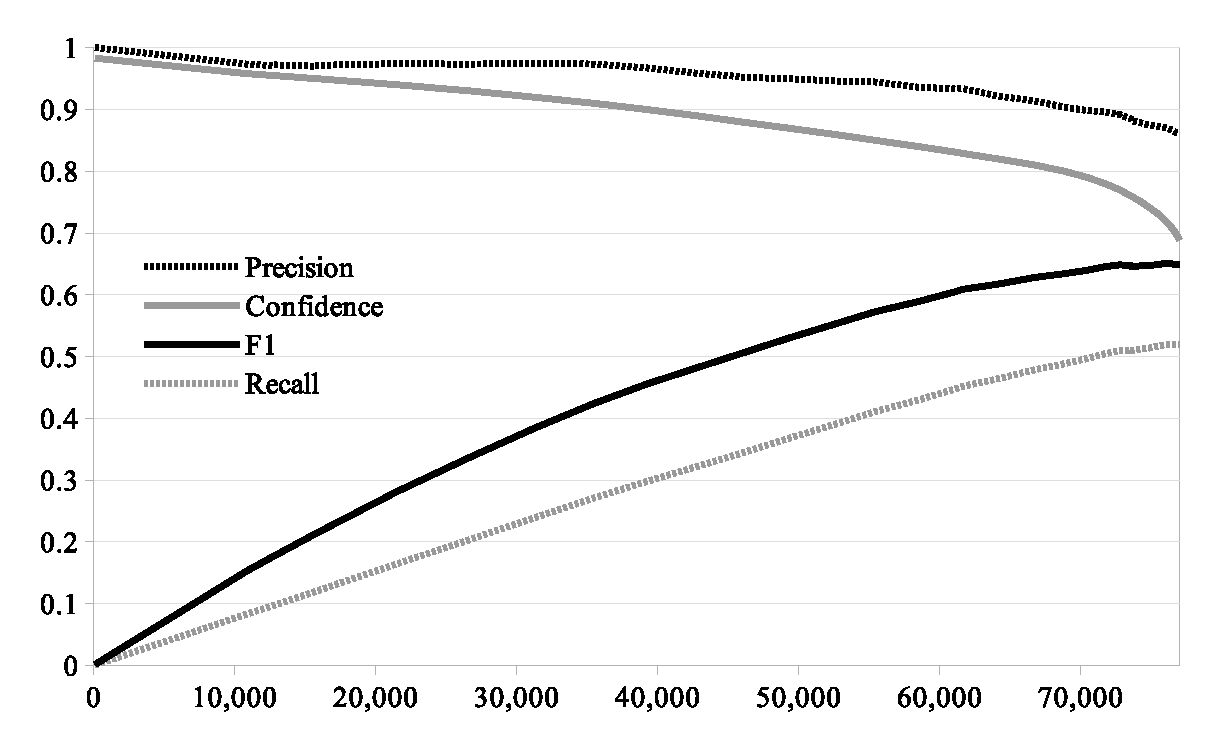
\includegraphics[width=\textwidth]{figures/curve.eps}
  \caption{\label{fig:curva}Average precision, recall, f-score, and confidence
    curves (from 0 to 1) versus total number of extractions of the \textsc{DiS} model.}
\end{figure}

%
\subsection{Error analysis}
\label{garcia:sec:error}
The manually annotated lists of bilingual collocations were used to perform an error analysis
of the \textsc{DiS} system. These errors were classified in five types depending on
their origin. \tabref{tab:error} contains, for each error type, the macro-average rates
of each \isi{collocation} pattern as well as the final distribution of the error typology.

\begin{enumerate}
\item \textbf{Bilingual model (\textit{BiModel}):} Though useful, the bilingual word embedding\is{word embeddings} approach
  produces some errors such as the identification of antonyms that have a similar distribution, which can align opposite \isi{collocation}
  equivalents, such as the Portuguese-English pair \ile{tecido\textsubscript{base} vivo\textsubscript{collocate}} = \ile{tissue\textsubscript{base} dead\textsubscript{collocate}}, instead of \ile{living tissue}, where the extracted equivalent of the collocate \ile{vivo} (\idio{living} -- in this context -- or \idio{alive}, in \ili{Portuguese})
  was \ile{dead}. In most cases, however, the system obtained similar
  (but not synonymous) collocations, such as \exidio{chá\textsubscript{base} preto\textsubscript{collocate}}{black tea} in Portuguese aligned to \exidio{coffee\textsubscript{base} black\textsubscript{collocate}}{black coffee} in English.

\item \textbf{Monolingual extraction (\textit{MonoExtract}):} The extraction of base and
  collocate pairs produced incorrect collocations such as
  \ile{plan\textsubscript{base} figure\textsubscript{collocate}},
  instead of obtaining the phrasal verb \ile{figure out} as collocate.  
  
\item \textbf{Preprocessing (\textit{NLP}):} Several errors derived from issues produced
  by the NLP pipeline, such as POS-tagging or dependency parsing:
  e.g., \textit{pain}\textsubscript{Noun},\\\textit{end}\textsubscript{Verb} was labeled
  as \textsc{dobj} (instead of \textsc{nsubj}).
  A special case of preprocessing errors was the analysis of some \ili{Portuguese}
  and \ili{Spanish} adverbs ending in \emph{--mente} (\emph{-ly} adverbs in \ili{English}),
  whose suffix was wrongly removed during the extraction process: e.g. \exidio{brutalmente}{brutally} $\rightarrow$ \ile{brutal}. These issues -- which can be easily corrected --
  caused the alignment of incorrect \ili{Spanish} and \ili{Portuguese}  collocations with
  \ili{English} candidates, such as the Portuguese-English pair \ile{matar\textsubscript{base} brutal\textsubscript{collocate}} = \ile{kill\textsubscript{base} brutally\textsubscript{collocate}} instead of \ile{matar\textsubscript{base} brutalmente\textsubscript{collocate}} = \ile{kill\textsubscript{base} brutally\textsubscript{collocate}}. This was the main source of errors of the \textsc{advmod} relation.

\item \textbf{Lemmatization and gender (\textit{Gender}):} The lemmatization of some words
  differs from language to language, so working with lemmas instead of
  tokens also might involve some errors. For instance, the Spanish word
  \exidio{hija}{daughter} is lemmatized as \exidio{hijo}{son}
  (also in \ili{Portuguese}: \ile{filha}, \ile{filho}), while in \ili{English} \ile{son}
  and \ile{daughter} appear as different entries. Thus, some bilingual
  collocations differ in the gender of their bases, such as the
  \ili{Spanish}-\ili{English} pair \ile{hijo\textsubscript{base} encantador\textsubscript{collocate}} = \ile{daughter\textsubscript{base} lovely\textsubscript{collocate}} instead of \ile{hijo\textsubscript{base} encantador\textsubscript{collocate}}=\ile{son\textsubscript{base} lovely\textsubscript{collocate}}.

\item \textbf{Other errors (\textit{Other}):} Some other errors were caused by mixed languages
  in the original corpus. For example, the verb form \ile{are}, in \ili{English}, was analyzed
  as a form of the verb \exidio{arar}{to plow} in \ili{Spanish}. Some errors also arose from noise
  and misspellings in the corpora (proper nouns with lowercase letters, etc.).
\end{enumerate}

It is worth mentioning that, in general, the error type distribution was similar across
the different \isi{collocation} patterns, showing much higher variation between different patterns
of the same language pair. For instance, the distribution of \ili{Spanish}-\ili{English} \textsc{amod} errors
is similar to the \ili{Portuguese}-\ili{English} \textsc{amod} one, while the typology of the \ili{Spanish}-\ili{Portuguese} \textsc{nmod}
errors is different to those of \ili{Spanish}-\ili{Portuguese} \textsc{amod} equivalents.

\begin{table}
  \begin{center}
    \caption{\label{tab:error} Error rate of each of the defined error types of \textsc{DiS} system (\emph{average} is macro-average).}
    \begin{tabular}{lrrrrrr}
      \lsptoprule
      \textbf{\emph{Type}}&\textbf{\textsc{amod}}&\textbf{\textsc{nmod}}&\textbf{\textsc{vobj}}&\textbf{\textsc{vsubj}}&\textbf{\textsc{advmod}}&\textbf{\emph{average}}\\
      \midrule
      \textbf{BiModel} & 70.57 & 93.52 & 59.23 & 45.74 & 32.61                 & 60.33\\
      \textbf{MonoExtract} & 0\phantom{00} & 0\phantom{00} & 21.43 & 21.85 & 44.94 & 17.64\\
      \textbf{NLP} & 8.34  & 0\phantom{00} & 16.96 & 11.48 & 20.49         & 11.45\\
      \textbf{Gender} & 21.10 & 2.78  & 2.38  & 19.07 & 0\phantom{00}         & 9.07\\
      \textbf{Other} & 0\phantom{00} & 3.70  & 0\phantom{00} & 1.85  & 1.96  & 1.50\\
      \lspbottomrule
    \end{tabular}
  \end{center}
\end{table}

Among the different errors produced by the presented method, an interesting case
are \emph{incongruent} collocations \citep{nesselhauf2003}. These expressions are
those where the translation of both elements is not coherent, such as the English-Portuguese pair \ile{requirement\textsubscript{base} meet\textsubscript{collocate}} = \ile{condição \textsubscript{base} cumprir\textsubscript{collocate}}, in which the verb \ile{to meet} is usually translated into \ili{Portuguese} as \ile{conhecer}, not as \ile{cumprir}.
For these \isi{collocation} equivalents to be correctly extracted by our method, they should
appear with some frequency in the training corpus, which is not always the case. This fact
may lead us to explore new compositional models, aimed at learning the distribution of the
whole \isi{collocation}, and not of its constituents, in further work.

\subsection{Comparable corpora}
A final experiment was carried out in order to find out (i) whether the bilingual
\isi{word embeddings} -- trained on the same \isi{parallel corpora} as those used for
extracting the collocations -- could be successfully applied to align collocations
obtained from different resources, and (ii) the performance of the proposed
method on comparable corpora.

Therefore, the same strategy for monolingual \isi{collocation} extraction was applied in the \ili{Spanish} and \ili{Portuguese}
\emph{Wikipedia Comparable Corpus 2014}.\footnote{\scriptsize{\url{http://linguatools.org/tools/corpora/wikipedia-comparable-corpora/}}}
Then, we calculated the semantic similarity between the collocations using the same word embedding\is{word embeddings}
models as in the previous experiments.

From these corpora, filtered lists of $89,285$ and $140,900$ candidate collocations in \ili{Portuguese}
and \ili{Spanish} were obtained, from 140M, and 80M of tokens respectively. From the $59,507$ bilingual
collocations obtained by the \textsc{DiS} approach, $150$ \ili{Spanish}-\ili{Portuguese} pairs were randomly selected
and evaluated.

The precision of the extraction was $87.25\%$, with a recall of $58.15\%$ (again computed
using the whole set of monolingual collocations), and $69.79\%$ f-score. These results are
in line with those obtained on the OpenSubtitles \ili{Spanish}-\ili{Portuguese} pair (about $2\%$ lower),
so the method works well on different corpora and domains. It is worth noting that
$49,259$ of the extracted \isi{collocation} equivalents ($83\%$) had not been retrieved from
the OpenSubtitles corpus.

This last experiment shows that (i) the bilingual \isi{word embeddings} can be used to identify
\isi{collocation} equivalents in different corpora than those used for training, and that
(ii) they can also be applied to corpora of different domains to obtain previously unseen
multilingual collocations.

%
\section{Conclusions}
\largerpage
\label{garcia:sec:conclusions}
This chapter presents a new strategy to automatically discover multilingual collocation
equivalents from both parallel and comparable corpora. First, monolingual collocation candidates of five different patterns are
extracted using syntactic analysis provided by harmonized UD annotation,
together with a combination of standard association measures. Besides, bilingual word embeddings are trained on lemmatized parallel corpora. These bilingual models are then
used to find distributional equivalents of both the base and
the collocate of each source collocation in the target language.

The performed experiments, using noisy parallel corpora in three languages,
showed that the proposed method achieves an average precision %in the bilingual alignment of collocations
of about $85\%$, with reasonable recall values.
A systematic comparison to translation dictionaries pointed out that
the distributional approach achieves similar precision results with much
higher recall values than the probabilistic dictionaries.
Furthermore, the evaluation showed that setting up a confidence value as
a threshold is useful for retaining only high-quality bilingual
equivalents, which could benefit the work on multilingual lexicography.

Finally, preliminary tests using comparable corpora suggested that
the bilingual word embeddings can be efficiently applied to different
corpora than those used for training, discovering new bilingual collocations
not present in the original resources.

The multilingual resources generated by the proposed method can be used in several
scenarios in which MWEs play an important role, such as machine
translation or second language learning. In this respect, corpora from various registers
and linguistic varieties could be used in order to obtain a wider diversity of collocation
equivalents that can be useful for different purposes.

The work presented in this chapter enables us to propose a number of directions for
further work. First, the results of the error analysis should be taken into account
in order to reduce both the issues produced by the NLP pipeline, and those
which arise from the word embedding models. On the one hand, understanding collocations
as directional combinations may lead us to evaluate other association measures
which are not symmetrical, e.g., \emph{Delta-P}. On the other hand, it could be
interesting to evaluate other approaches for the alignment of bilingual collocations
which make use of better compositionality models, and which effectively learn the semantic
distribution of collocations as single units, in order to deal with cases of incongruent
collocation equivalents.


\begin{section}*{Abbreviations}
    \begin{tabularx}{.49\textwidth}{ll}
      \textsc{em} &   expectation maximization    \\
      \textsc{en} &   English    \\
      \textsc{mi} & mutual information    \\      
      \textsc{mwe} &  multiword expression  \\            
       \end{tabularx}
      \begin{tabularx}{.49\textwidth}{ll}      
      \textsc{nlp}  & natural language processing\\
      \textsc{pt} &  Portuguese    \\
      \textsc{es} &   Spanish    \\      
      \textsc{ud} &     Universal Dependencies  \\
    \end{tabularx}
\end{section}


\section*{Acknowledgements}
\largerpage
This work has been supported by the Spanish Ministry of Economy, Industry and
Competitiveness through the project with reference FFI2016-78299-P,
by two \emph{Juan de la Cierva} grants (FJCI-2014-22853 and IJCI-2016-29598),
and by a 2017 Leonardo Grant for Researchers and Cultural Creators, BBVA Foundation.

{\sloppy
\printbibliography[heading=subbibliography,notkeyword=this]
}

\end{document}
